% word limit: 500
\section{Results}

To explore the shape of the rotation period-\teff\ relation, we selected
groups of stars within different age ranges, and calculated the velocity
dispersion, $\sigma_{v{\bf b}}$ as a function of effective temperature for
each group.
We chose to use effective temperatures and not colors in this analysis as it
is the linear quantity and therefore easier to divide into bins of roughly
equal numbers of stars.
Ages were calculated with the \citet{angus2019} gyrochronology relation, which
is based on Praesepe and the Sun and calibrated in \gaia\ \gcolor\ color.
This relation was calibrated by fitting a 5th-order polynomial to the relation
between rotation period and \gaia\ \gcolor\ color for around 800 members of
the Praesepe cluster, and a straight line in age to Praesepe and the Sun.
Although only calibrated using Praesepe and the Sun, this gyrochronology
relation was tested on NGC 6819, a 2.5 Gyr cluster, and predicted accurate
ages for members of that cluster.
In addition, the period-color relation of Praesepe is nearly identical to the
period-color relation of the Hyades, a cluster of around the same age: $\sim$
650 years \citep{douglas2019}.
However, this relation does {\it not} provide a good fit to NGC 6811, a 1.1
Gyr cluster \citep{curtis2019}.
The G dwarfs in this cluster rotate at the same rate as the K dwarfs.

The \citet{angus2019} gyrochronology relation assumes that the rotation
period-color relation of Praesepe is applicable to stars of all ages: the same
polynomial relation fit to Praesepe is used to describe the period-color
relation at all ages.
If the rotation-color relation of the \citet{angus2019} gyrochronology
relation were a perfect model for the rotational evolution of stars, then
groups of stars selected to be similar ages using this relation should fall on
an isochrone on both a CMD, and in period-\teff\ space.
Unfortunately, uncertainties on \gaia\ photometry and parallaxes, plus
metallicity and extinction blur out the main sequence enough that differences
between stars in different age and rotation bins are not easily discernable on
the CMD, although there is still a general age and rotation period gradient on
the CMD, as seen in figures \ref{fig:CMD_cuts} and \ref{fig:age_gradient}.
\begin{figure}
  \caption{
Main sequence stars with \mct\ rotation periods on the \gaia\ CMD with visual
    binaries removed.
    Points are colored by their gyrochronal age, according to the
    \citet{angus2019} gyrochronology relation.
    A general age gradient is visible across the main sequence.
}
  \centering
    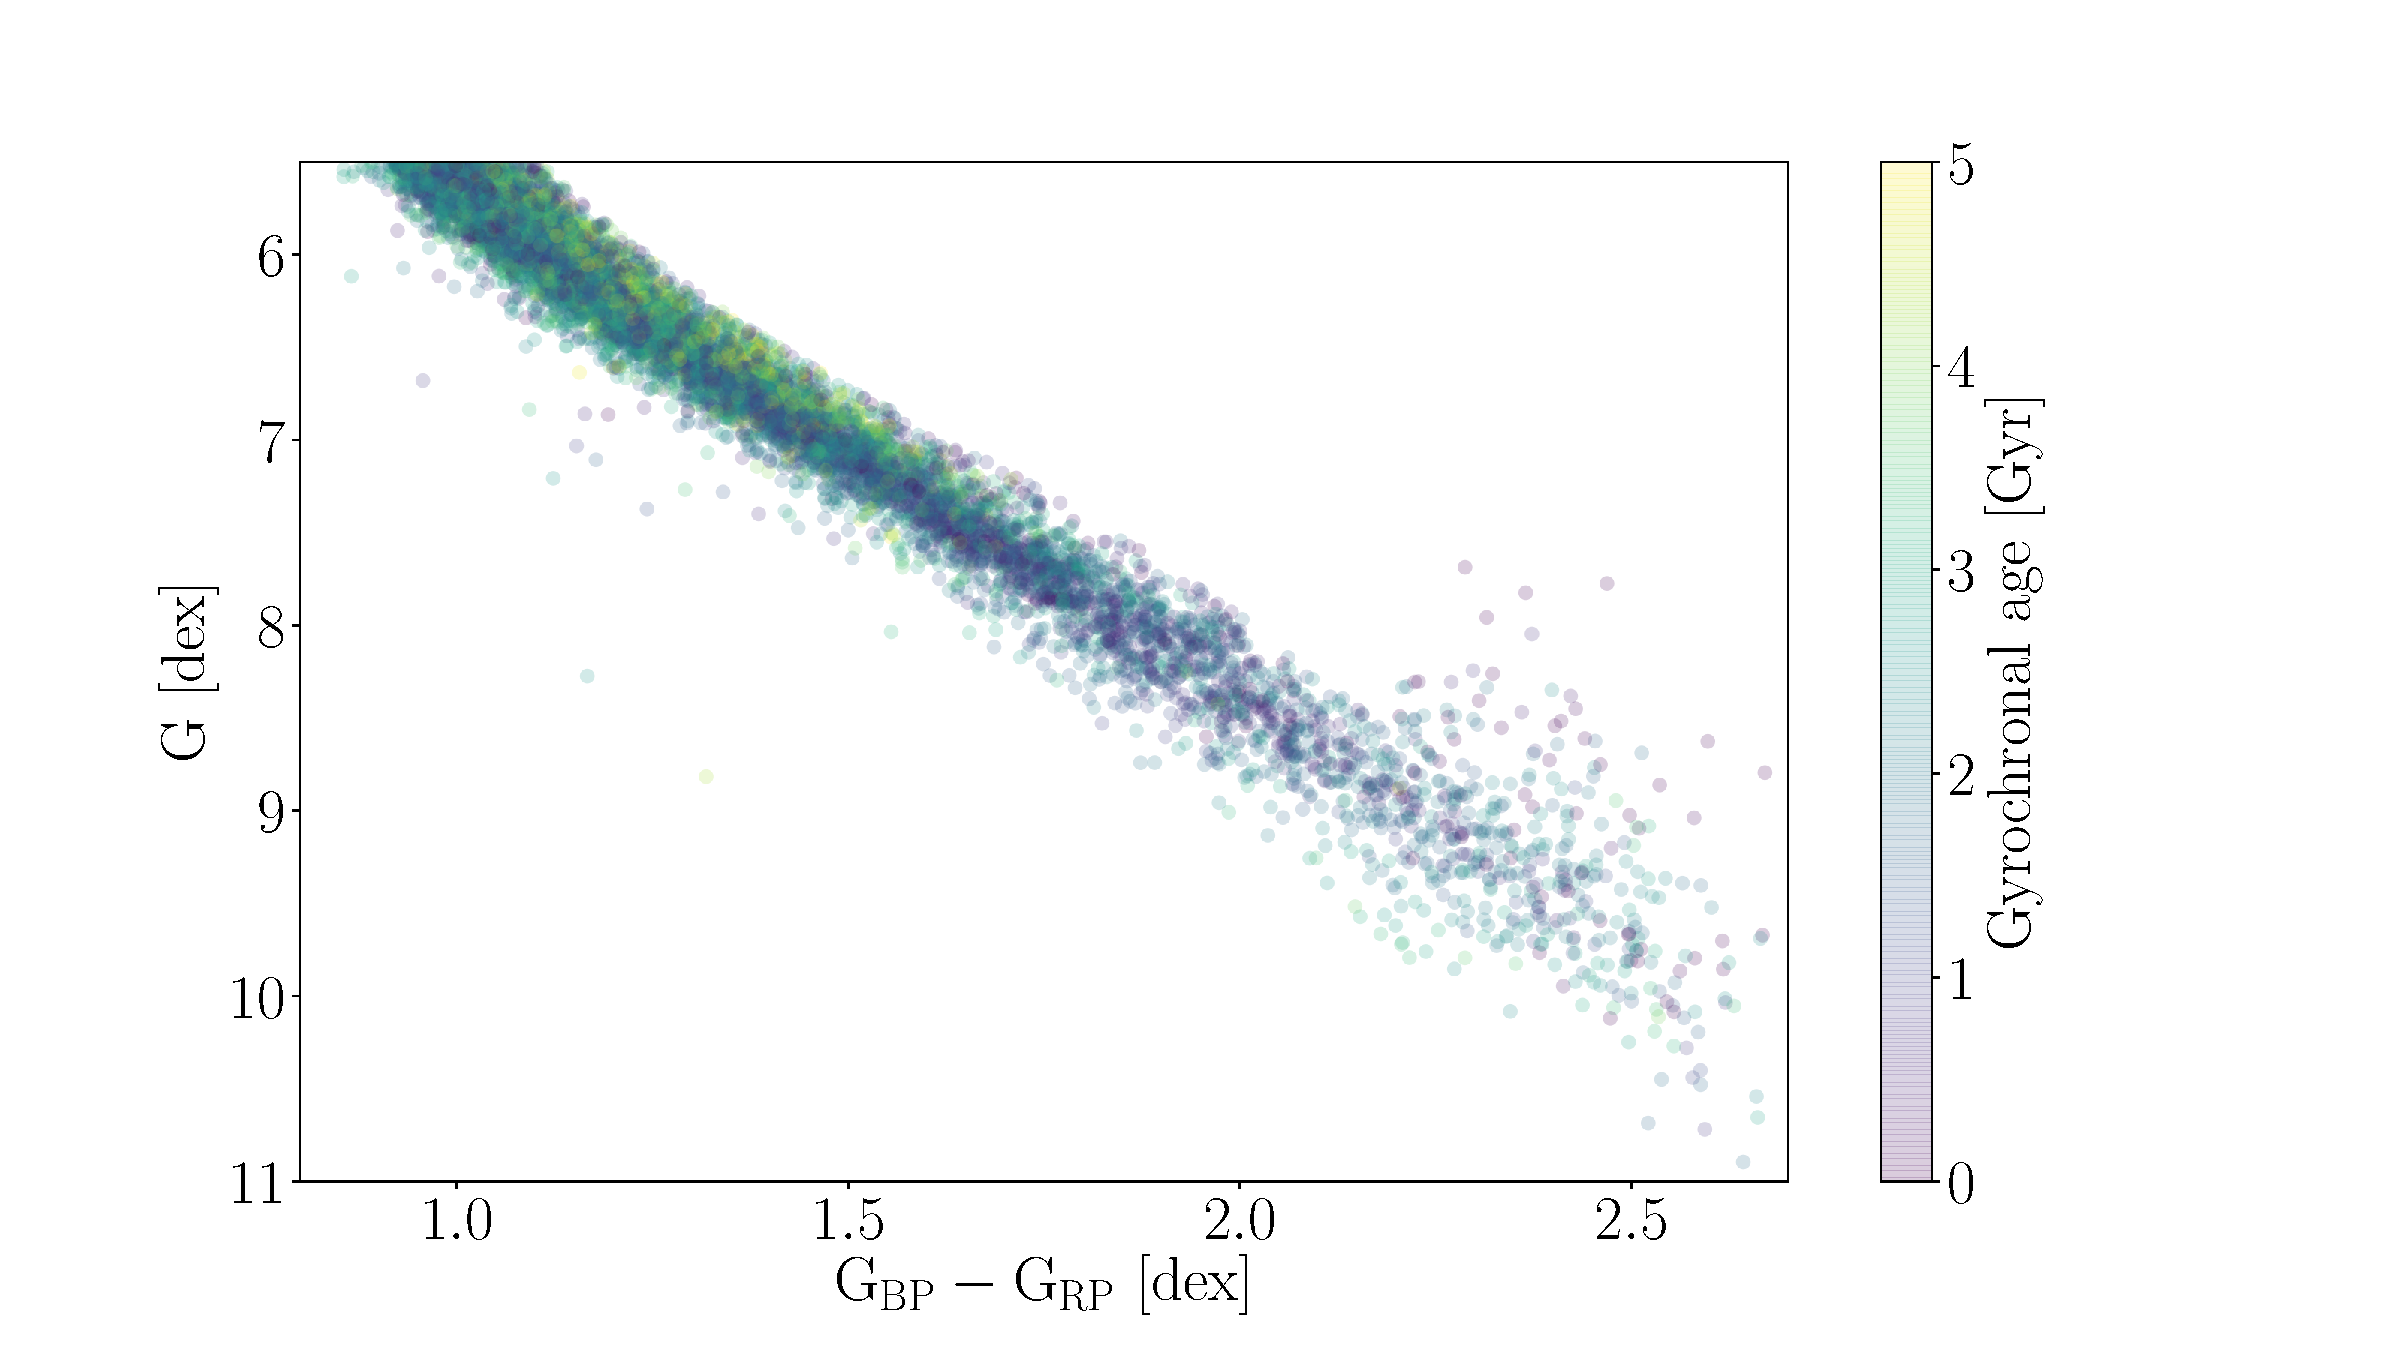
\includegraphics[width=1\textwidth]{age_gradient}
\label{fig:age_gradient}
\end{figure}
In contrast, isochrones and stellar evolution tracks are highly dependent on
choices made about input physics and assumptions and have often been
calibrated using different types of stars.
As a result, different sets of models can have very different shapes on the
CMD, particularly at low masses.
Instead of relying on CMD position to age-date groups of stars, we opted to
explore age trends via kinematics.
Kinematic age-dating has the advantage of being relatively model independent,
or at least, having a very simple model: that velocity dispersion increases
over time.
This means that it is relatively easy to rank groups of stars by age: older
groups have a larger velocity dispersion.
It is less easy to rank-order groups of stars by age on the CMD because
stellar evolution is highly mass and metallicity dependent, and because
different stellar evolution models predict different ages for the same CMD
position.
This does not mean that it is not possible to calibrate gyrochronology using
isochrones, however we leave this exercise for a future study.

\subsection{Selecting groups of stars to examine the gyrochronology relations}

In order to examine the rotation period-temperature/color relation, we
selected stars in the \mct\ sample with the same gyrochronal age, calculated
using the \citet{angus2019} relations.
The top panel of figure \ref{fig:age_cut} shows the full \mct\ sample (minus
visual binaries and subgiants) in grey, with groups selected by age shown in
color.
The bottom panel shows the velocity dispersion of each age group, as a
function of effective temperature.
If the stars in each group have the same age across the temperature range,
their velocity dispersion should be constant.
Although the youngest age groups have a relatively constant velocity
dispersion across temperatures, the oldest age groups do not.
This indicates that the shape of the period-color relation does not remain
constant over time -- it flattens out.
In the oldest age bin, the cool stars have a larger velocity dispersion than
the hot stars, suggesting that the cool stars are older than the hot stars
(\ie\ these stars do not actually belong in the same age bin).
Either the cool stars are being grouped into an age bin that is too young, or
the hot stars are grouped into an age bin that is too old, but either way, the
isochrones used to make the age selection are too steeply sloped.
\begin{figure}
  \caption{
Top: rotation period vs effective temperature for stars in the \mct\
    catalog.
    The full catalog, with subgiants and visual binaries removed is shown in
    grey, and stars selected to be in different age groups are overlayed in
    color.
    These age groups were selected using the \citet{angus2019} gyrochronology
    relation.
The legend in the center of the figure lists the age range of each group.
    Bottom: velocity dispersion vs effective temperature for each age group.
The color of the line corresponds to the color of the group shown in the top
    panel.
If the gyrochronal model were correct at all ages and the stars in each group
    were the same age across temperatures, the velocity dispersion would be
    constant as a function of \teff.
However, the velocity dispersions of the oldest age groups depend on \teff,
    indicating that the \citet{angus2019} gyrochronology model either
    overpredicts the ages of old M dwarfs or underpredicts the ages of old G
    and K dwarfs.
}
  \centering
    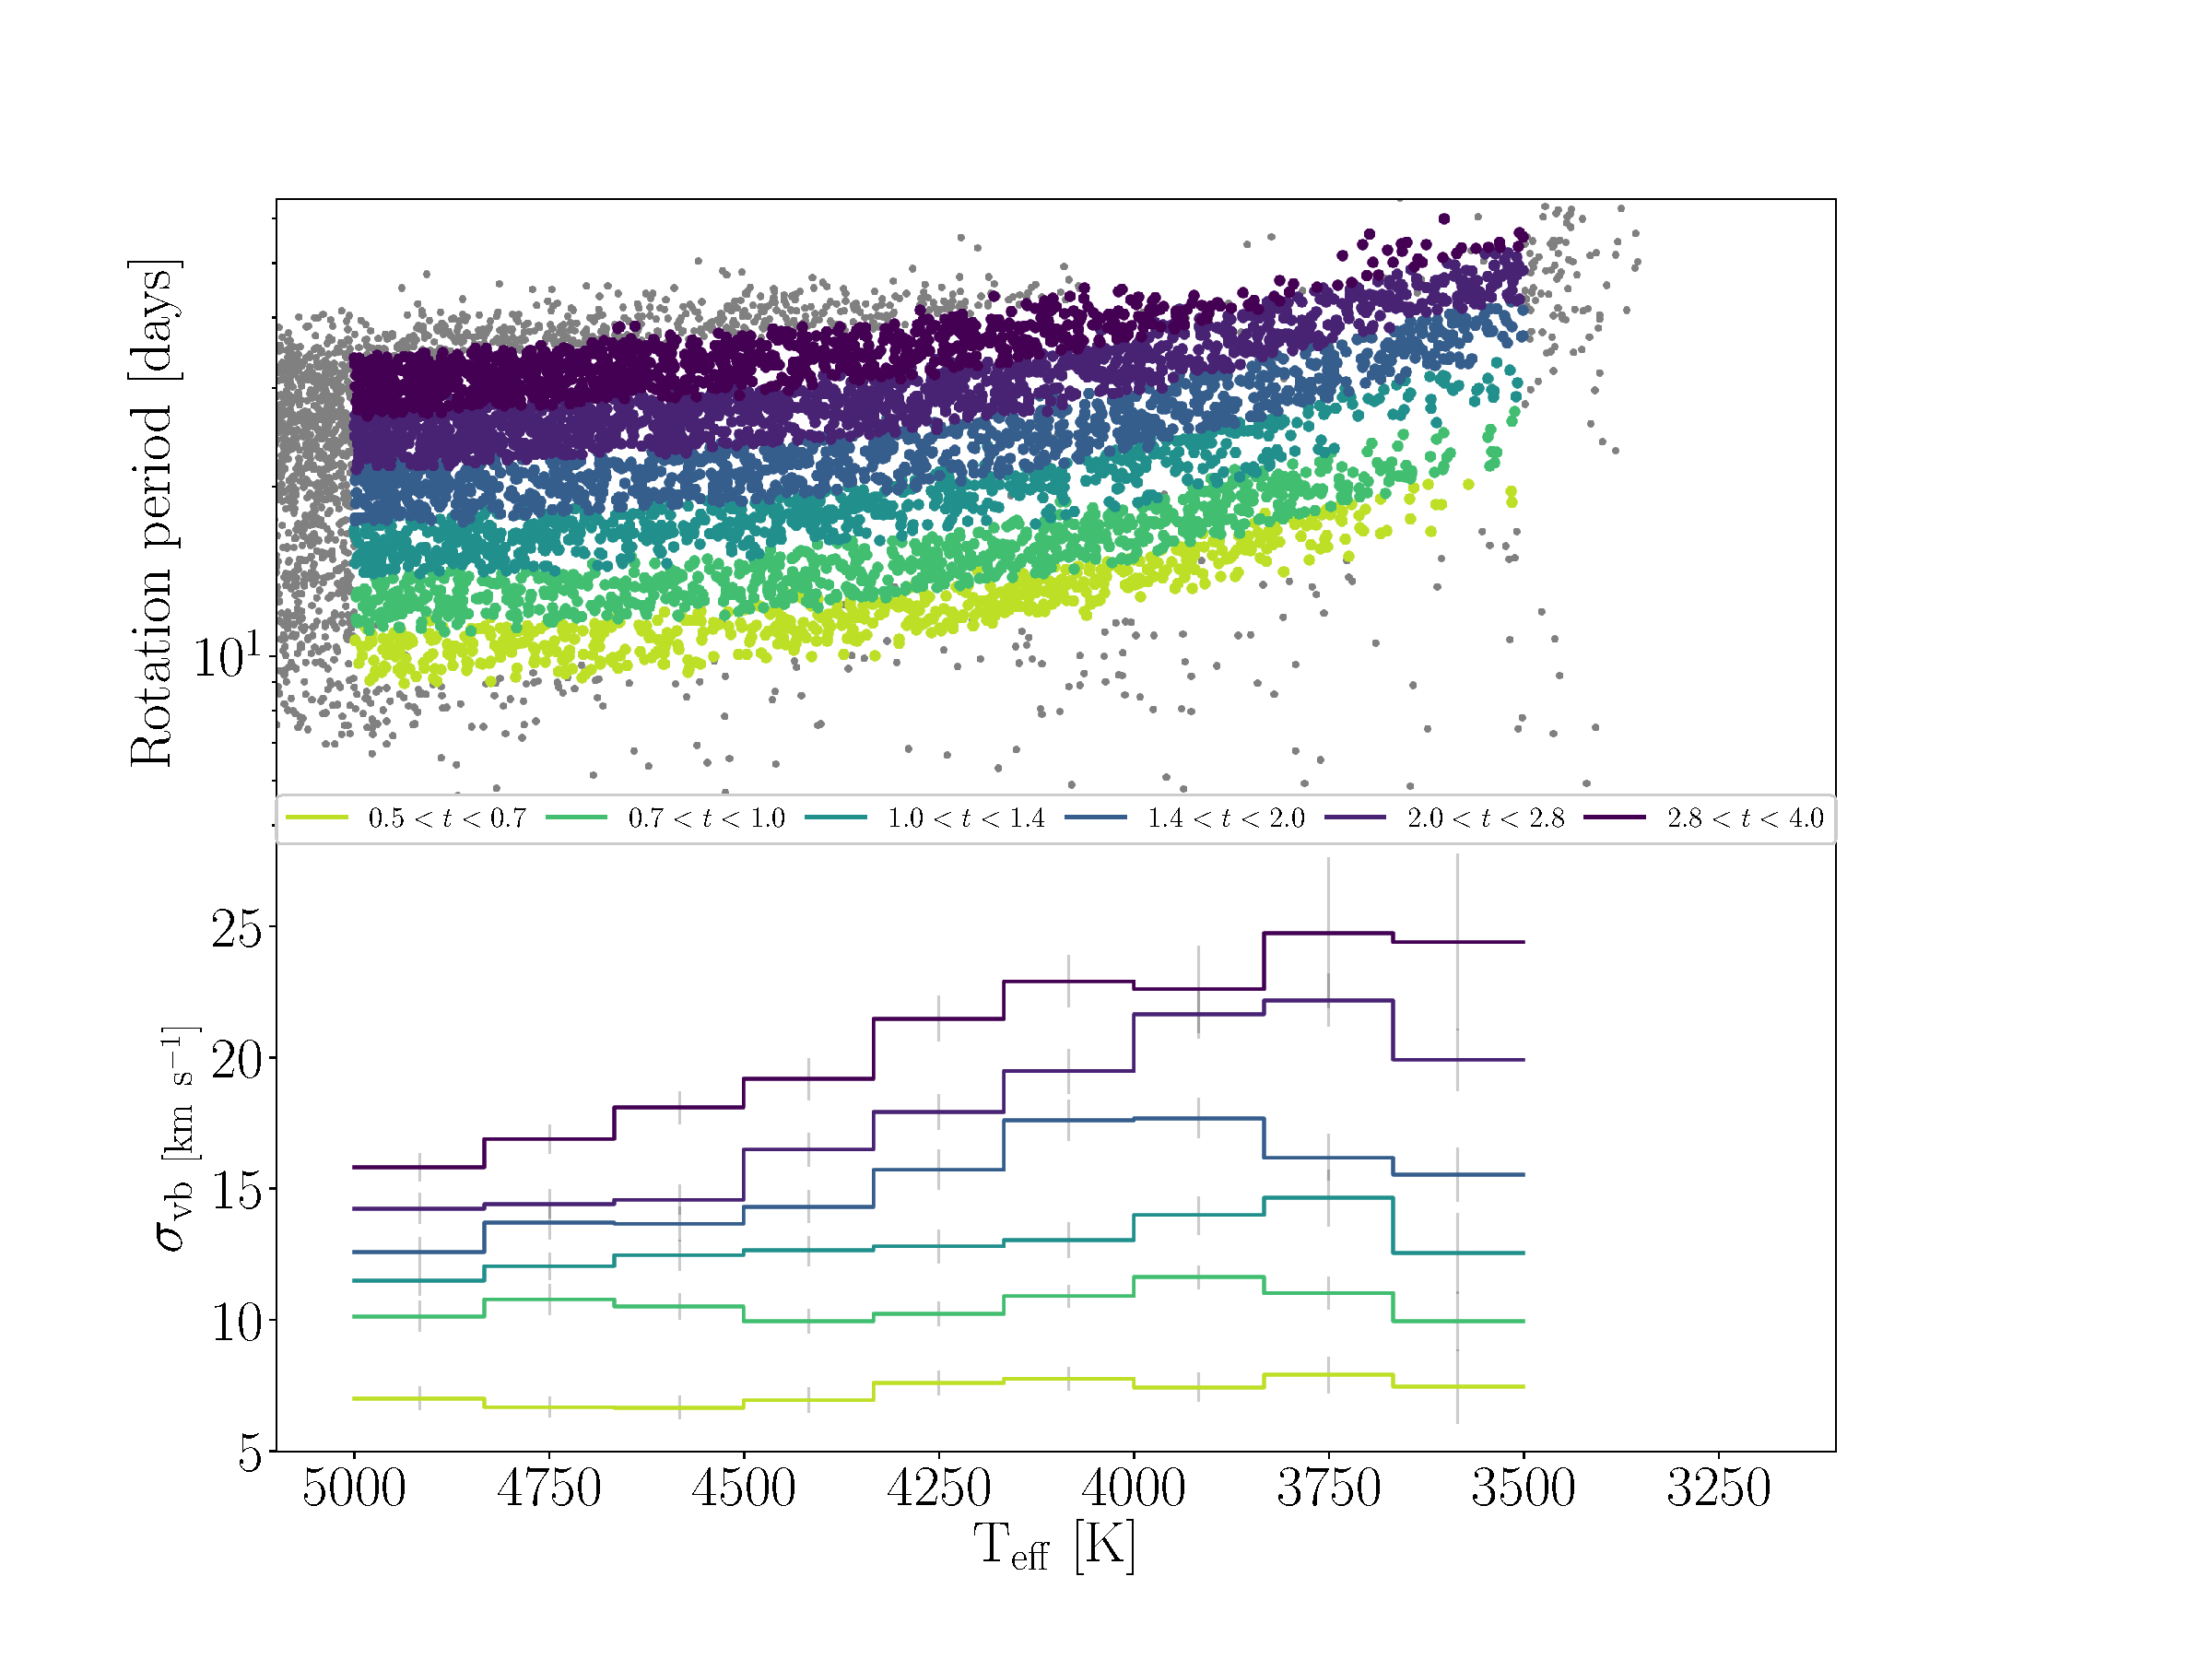
\includegraphics[width=1\textwidth]{age_cut}
\label{fig:age_cut}
\end{figure}

We applied the same analysis to groups of stars selected using simple rotation
period cuts.
The top panel of figure \ref{fig:period_cut} shows the \mct\ sample with
selected groups of stars shown in different colors.
The bottom panel shows the velocity dispersion as a function of effective
temperature for each group.
\begin{figure}
  \caption{
This figure is similar to figure \ref{fig:age_cut}, with stars divided into
    period groups rather than age groups.
The velocity dispersion is more constant across effective temperatures for the
    most slowly rotating stars, compared to the stars selected with the
    \citet{angus2018} gyrochronology model.
    This indicates that the gyrochronology models flatten out, and possibly
    even invert, at old ages.
}
  \centering
    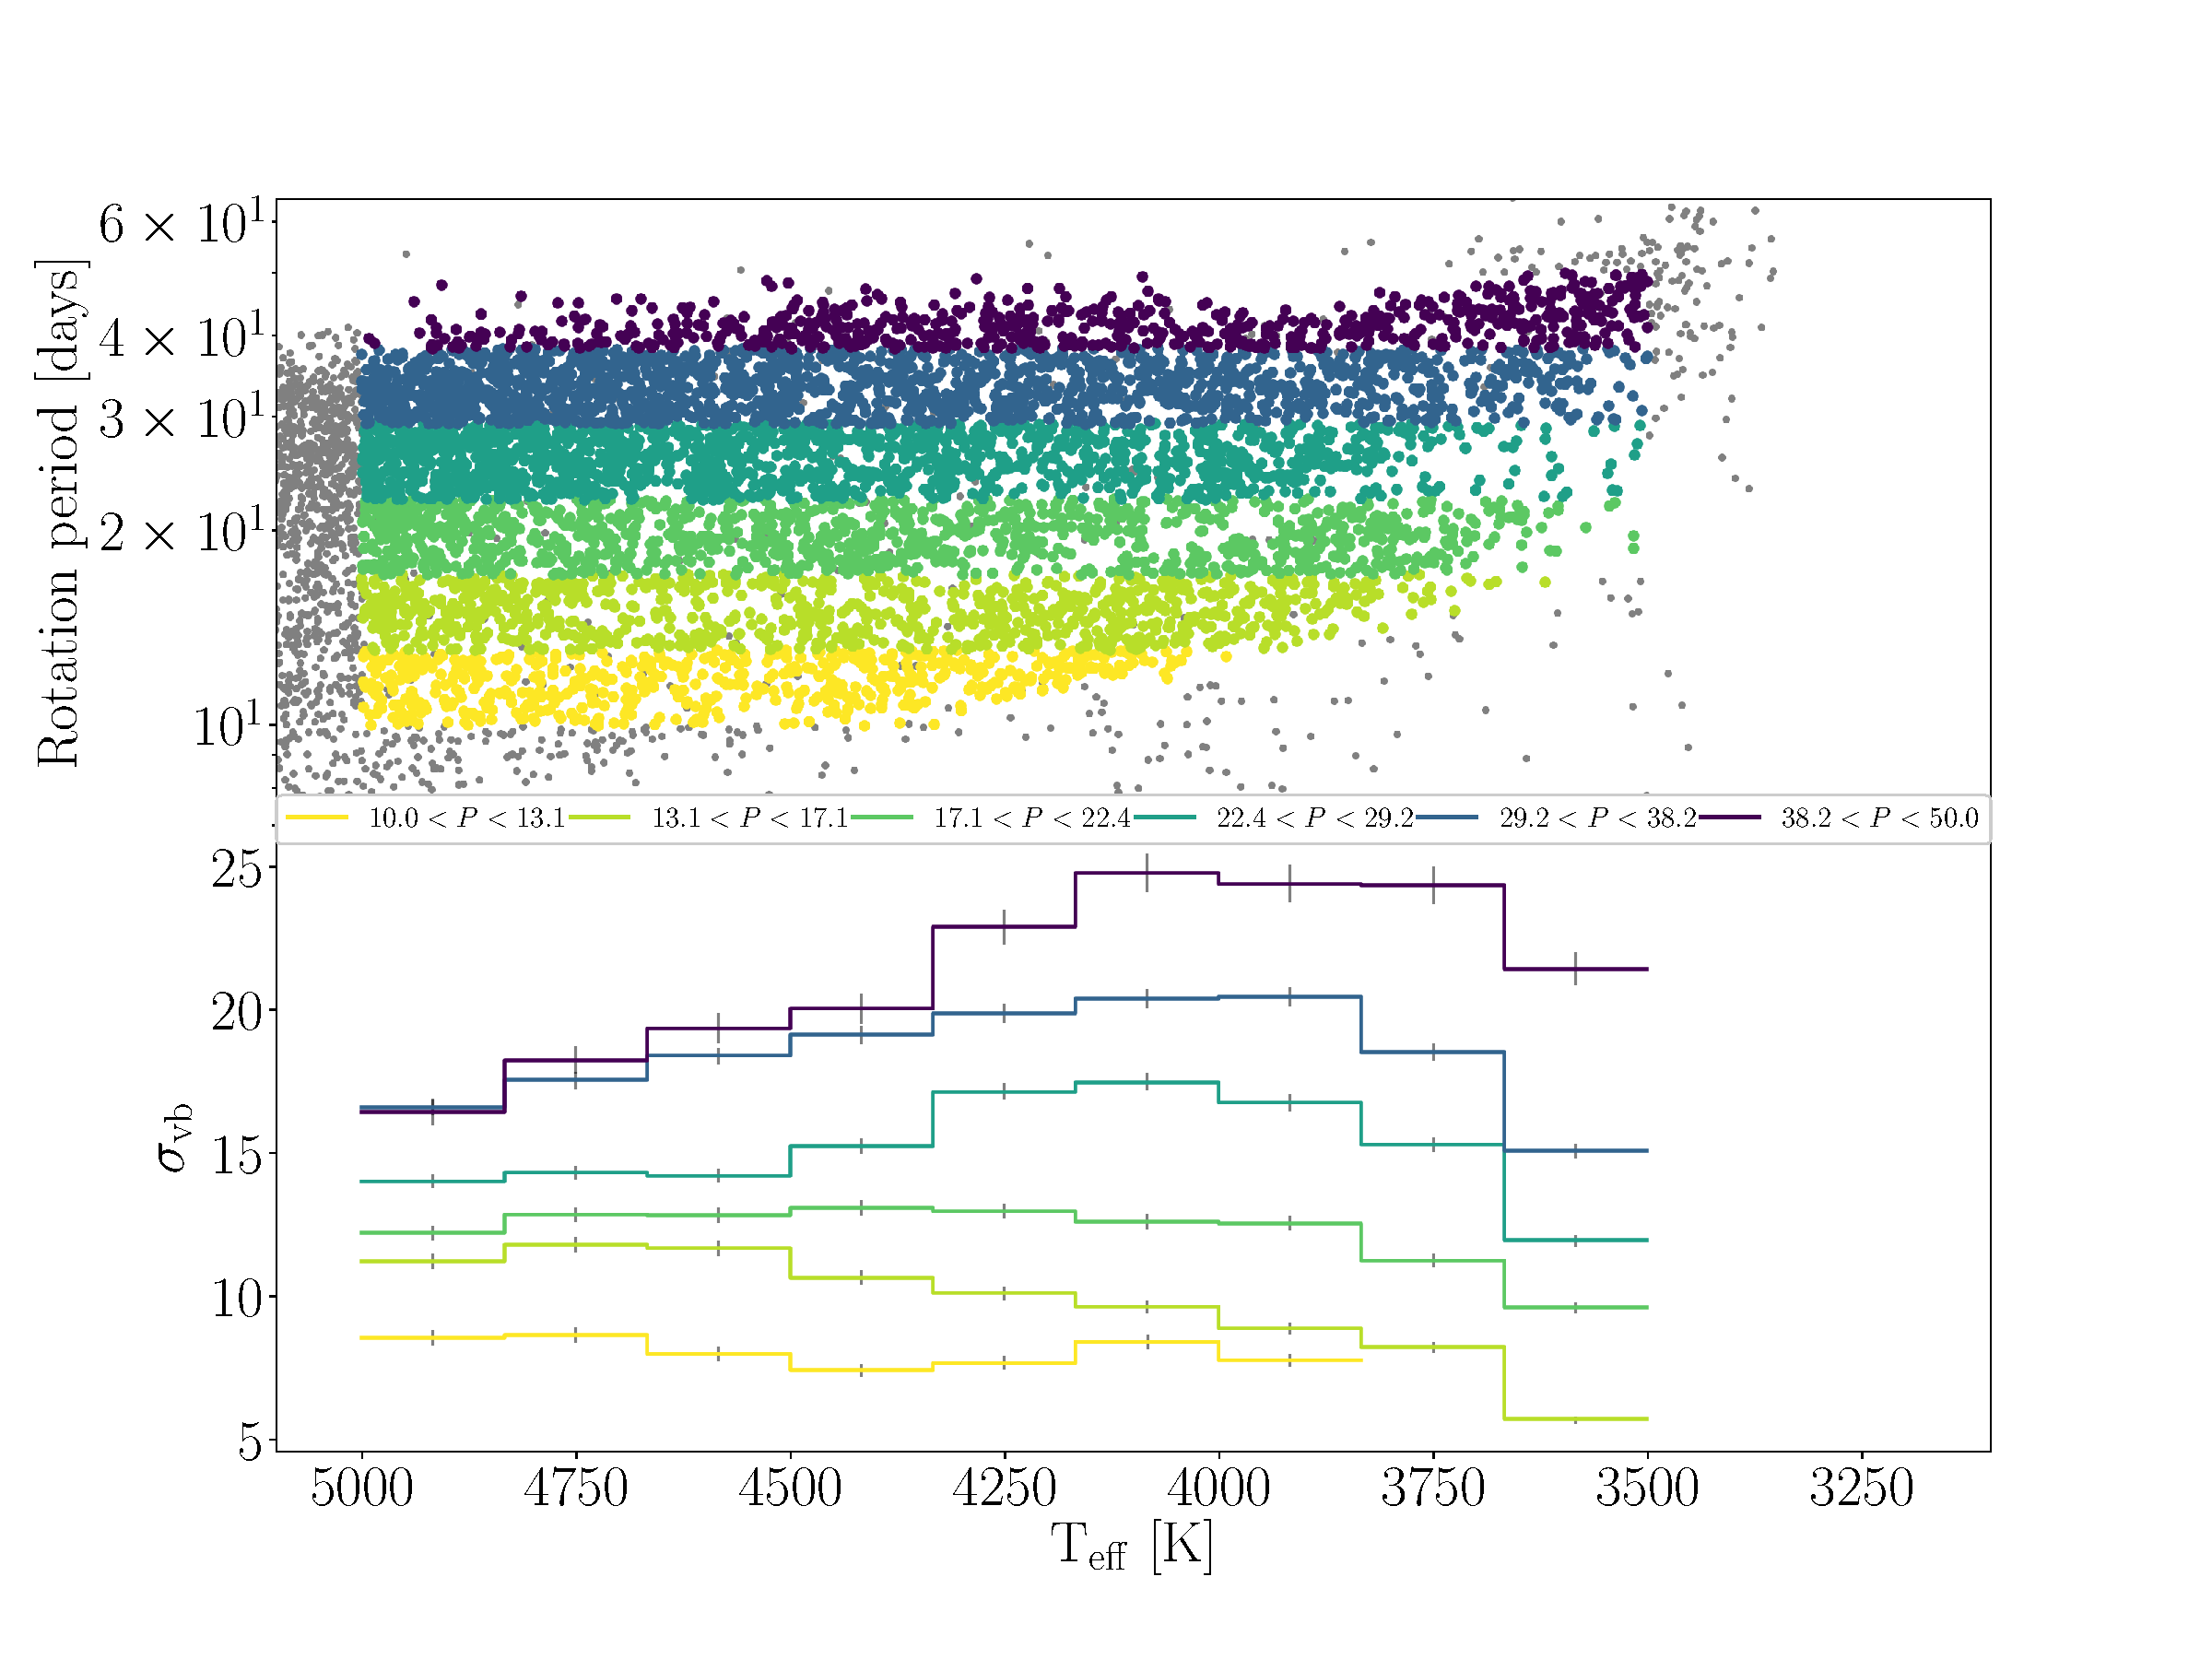
\includegraphics[width=1\textwidth]{period_cut}
\label{fig:period_cut}
\end{figure}

% \begin{figure}
%   \caption{
% Rotation period vs. velocity in the galactic latitute direction.
% }
%   \centering
%     \includegraphics[width=1\textwidth]{rotation_vb_dispersion}
% \label{fig:rotation_vb_dispersion}
% \end{figure}

% \begin{figure}
%   \caption{
% Age vs. velocity in the galactic latitute direction.
% The velocity of stars as a function of their age.
% }
%   \centering
%     \includegraphics[width=1\textwidth]{age_vb_dispersion}
% \label{fig:age_vb_dispersion}
% \end{figure}

% figure \ref{age_vb_dispersion} shows the velocity of stars in the \bvector\
% direction, plotted against their gyrochronal ages.
% These ages were calculated using equation 1 of \citet{stardate_paper},
% implemented in the \sd\ \python\ package \citep{stardate}.
% The two vertical lines show the approximate locations of the synchronized
% binary upper limit and the rotation gap.
% Stars to the left of the rotation gap (age $\lesssim$ 1 Gyr) and to the right
% of the synchronized binary regime (age $\gtrsim$ 0.5 Gyr) have lower $V_b$
% dispersion than stars to the right of the rotation gap (age $gtrsim$ 1 Gyr),
% indicating that they are kinematically young.
% This increase in velocity dispersion can be seen in both the individually
% plotted stars, and in the bins of standard deviation shown as the solid black
% line, which increase with age.
% This figure clearly indicates that stars with rotation periods that indicate
% they are young (but are greater than 7 days), are indeed young.
% This rules out the possibility that the rotation period gap is caused by
% either incorrect rotation periods, or binarity.

% This figure also shows a lack of M dwarfs at old ages caused by the `M dwarf
% dip' \citep{vansaders2019, mcquillan2014}.
% This is a feature of the \citet{mcquillan2014} sample where there appears to
% be a lack of slowly rotating stars at temperatures cooler than 4000 K.
% Like the rotation period gap, the origin of the M dwarf dip could either be
% due to a lack of stars with long rotation periods, or due to a suppression in
% the amplitudes of variability for these stars.
% However, in general the completeness of the \citet{mcquillan2014} catalog
% increases as a function of decreasing temperature, and is around 80\% for M
% dwarfs \citep{mcquillan2013, mcquillan2014, simonian2019}.
% This suggests that the age-rotation relation has a different shape at
% different ages, as indicated by the 1 Gyr NGC 6811 cluster that has a
% different rotation period-age relation to those of younger clusters
% \citep{curtis2019}.
